\section{Background}
\label{sec:background}

\gls{nso} foundations can be rooted back to three enabling technologies, namely Cloud Computing, SDN, and NFV. This section provides a brief background on these topics and their relationships to NSO, in addition to a short historical review of the term ``orchestration''.

\subsection{Cloud Computing}
Cloud computing is a model for providing resource virtualization (e.g., networks, servers, storage, and services) with high flexibility, cost efficiency, and centralized management~\cite{Le2016SurveyNetworks}. The cloud computing service models are generally categorized in \gls{iaas}, \gls{paas}, and \gls{saas} which offer, respectively,  virtual resources (compute, storage, and network), software and development platforms (provided by the cloud infrastructure), and Internet-based applications (hosted on the cloud)~\cite{bele2018empirical}.

%Cloud computing is a model for enabling ubiquitous, convenient, on-demand network access to a shared pool of configurable computing resources (e.g., networks, storage, and services) that can be rapidly and automatically provisioned and released with minimal effort~\cite{Mell2011TheTechnology}. Thereby, the resources are traded on demand, that is, the customer only pays what is used. Cloud computing becomes one of the relevant technology for the 5G networks mainly because it provides high data rate, high mobility, and centralized management \cite{Le2016SurveyNetworks}.

%The service models of cloud computing  are generally categorized into three classes: \gls{saas}, \gls{paas}, and \gls{iaas}. In a cloud \gls{iaas}, the infrastructure is offered as a service to the customer. Each customer can have its virtual resources, such as compute, storage, and network. 
%\gls{saas} includes applications such as Facebook, Google Apps, Twitter, and Microsoſt Office 365.

%\gls{paas} provides services according to a user’s applications without installing or configuring the operating system. The customers can develop and deploy their applications in the same development environment. The \gls{paas} model includes services such as Microsoft Azure, Google App Engine, RedHat OpenShift, and Amazon Elastic Beanstalk.  

%In \gls{saas}, in turn, the customer is able to use the providers' applications running on a cloud infrastructure~\cite{Mijumbi2016NetworkChallenges}. The softwares are maintained and managed by a cloud provider. \gls{iaas} includes applications, for example, OpenStack, CloudStack, Amazon CloudFormation, and Google Compute Engine.

In a cloud environment, the notion of orchestration has also been used for integrating basic services~\cite{Vouk2008CloudImplementations}. The Orchestration in the cloud involves dynamically deploying, managing and maintaining resource and services across multiple heterogeneous cloud platforms in order to meet the needs of clients. 
%This procedure demands to automatize processes and create a workflow.
%However, this is not a simple task.

%The Cloud computing service layers are depicted in Figure~\ref{cloud}
% \begin{figure}[thpb]
%   \centering
%   \includegraphics[scale=.36]{Figures/02_Background/cloud2}
%     \caption{Cloud computing service layers.}
%     \label{cloud}
% \end{figure}


%Diference between cloud and nfv. See slide 60,68 NFV
%https://sdn.ieee.org/newsletter/september-2017/intent-based-management-and-orchestration-of-heterogeneous-openflow-iot-sdn-domains
\subsection{Software Defined Networking (SDN)}
%Software-defined networking
%Software Defined Networking
%Software Defined Network

%SDN~\cite{kreutz2015software} is an emerging networking paradigm that attempts to resolve the strongly vertical integration of current network environments. To do so, SDN proposes to decouple the control plane from the data plane (See Fig. x). With this new architecture , data forwarding equipments (e.g. routers and switches) become simple forwarding network elements whose control logic is provided by a external entity called SDN controller or network operating system (NOS). In the upper layer, software network customized applications 
%is used to provide  abstract the lower-level functionalities and  

\gls{sdn}~\cite{surveySDN} is an evolving networking paradigm that attempts to resolve the strongly vertical integration of current network environments. To this end, \gls{sdn} proposals decouple the control plane (i.e., control logic) from the data plane (i.e., data forwarding equipment). With this new architecture, routers and switches become simple forwarding network elements whose control logic is provided by an external entity called \gls{sdn} controller or \gls{nos}. 

\glspl{nbi} offered by a logically centralized \gls{sdn} controller allow different network applications (firewalls, routing, and resource orchestrators) to implement network control and operation logic. In addition, other type of high-level \acrshortpl{nbi} category are implemented as \gls{nos} management applications~\cite{Rotsos2017NetworkSurvey}. Examples of this category include Virtual Tenant Networks, \gls{alto}, and Intent-based networking (IBN).

%Service orchestrators, OSSes and other network applications can be developed on top of high-level \glspl{nbi} offered by a logically centralized \gls{sdn} controller. Indeed, \acrshortpl{nbi} are crucial components to control and monitor the network services orchestration.

%The logically centralized \gls{sdn} controller acts in spirit of computer operating systems that provide a high-level abstraction for the management of computer resources (e.g., hard drive, CPU, memory) by playing the network operating system role for network management~\cite{gude2008nox}. As such, it provides a set of services (base network services, management, orchestration) and common interfaces (North/South/East/West) to developers who can implement different control applications and improve manageability of networks. Moreover, such interfaces are used within the \gls{mano} framework to deploy end-to-end connectivity. As today, the most popular open source \gls{sdn} controllers are \gls{onos}~\cite{ON.LABONOSScale-out.} and OpendayLight~\cite{LinuxFoundationOpenDaylight}.


%Service orchestrators, OSSes and other network applications can be developed on top of high-level \glspl{nbi} offered by a \gls{sdn} controller. %Indeed, \acrshortpl{nbi} are crucial components to control and monitor the network services orchestration.

%The \gls{sdn} controller creates an abstract network view while hiding details of the underlying physical or virtual infrastructure. Running on the top of the \gls{sdn} controller, software network applications can perform not only traditional functionalities such as routing, load balancing, classification~\cite{6965141}, or \acrlongpl{ids}, but also propose novel use cases such as service  orchestration across multi-domain and multi-technology in 5G networks~\cite{Bernardos20155GInfrastructures}. Those applications, together with others industry and academy initiatives towards flexible network services over programmable resources are, among the main drivers of \gls{sdn}.

%Service orchestrators, OSSes and other network applications can be developed on top of high-level \glspl{nbi} offered by a \gls{sdn} controller. Indeed, \acrshortpl{nbi} are crucial components to control and monitor the network services orchestration. Unlike \acrshortpl{sbi}, where Openflow is a well-known \gls{sdn} standard protocol, \acrshortpl{nbi} are still an open issue with different controllers offering a variety of \acrshortpl{nbi} (e.g., RESTful APIs~\cite{richardson2008restful}, NVP NBAPI~\cite{onix},~\cite{koponen2014network}, SDMN API~\cite{pentikousis2013mobileflow}, etc.). In addition, other type of high-level \acrshortpl{nbi} category are implemented as \gls{nos} management applications~\cite{Rotsos2017NetworkSurvey}. Examples of this category include Virtual Tenant Networks, ALTO, and Intent-based networking (IBN).

%The communication between the \gls{sdn} controller and the forwarding devices is done through \glspl{sbi}, which allow decoupling the control and data plane via open communication protocols (i.e. well-defined APIs). Different \gls{sdn} \glspl{sbi} can be considered (e.g., ForCES~\cite{Doria2010}, OVSDB~\cite{Davie2013RFCProtocol}, POF~\cite{song2013protocol}, etc.), with  OpenFlow~\cite{openFlow},~\cite{SDXCentral2014WhatAPIs} being the most widely accepted solution available in commercial and open source (hardware and software) devices.  %The Openflow protocol provides three major informations for the SDN controller: (i), (ii), (iii)
%are enabling  providing customized and optimized network services 
%%and Robert Szabo  
%Software defined networking is a computer networking approach that lets network administrators manage network services through abstraction of lower-level functionality. SDN decouples the control plane (controllers and/or Network Operating Systems) from the data plane (equipments to forwarding of data) \cite{c7}[rever].
%SDN addresses the challenge that the static architecture of traditional networks does not support the scalable, dynamic computing and storage needs of dynamic environments, e.g. datacenter and operator networks. It creates an abstract vision of network that enable fast innovation and networks more agile and flexible.

%Service orchestrators, OSSes and other network applications can be developed on top of high-level \glspl{nbi} offered by a \gls{sdn} controller. Indeed, \acrshortpl{nbi} are crucial components to control and monitor the network services orchestration. Unlike \acrshortpl{sbi}, where Openflow is a well-known \gls{sdn} standard protocol, \acrshortpl{nbi} are still an open issue with different controllers offering a variety of \acrshortpl{nbi} (e.g., RESTful APIs~\cite{richardson2008restful}, NVP NBAPI~\cite{onix},~\cite{koponen2014network}, SDMN API~\cite{pentikousis2013mobileflow}, etc.). In addition, other type of high-level \acrshortpl{nbi} category are implemented as \gls{nos} management applications~\cite{Rotsos2017NetworkSurvey}. Examples of this category include Virtual Tenant Networks, ALTO, and Intent-based networking (IBN).% However, initiatives such as the ONF's NBI working group are making good progress developing an intent-based interface~\cite{OpenNetworkingFoundation2017Intent:BLOG},~\cite{NetworkComputing2015SDNsEvolves} which is expected to become a common interface to applications and services.% An orchestrator uses NBIs and the VNF Manager () to 

%http://www.networkcomputing.com/networking/sdns-northbound-interface-evolves/562466230
%https://www.opennetworking.org/?p=1633&option=com_wordpress&Itemid=155
%https://www.sdxcentral.com/articles/contributed/intent-based-networking-seeks-network-effect-david-lenrow/2015/09/

%The logically centralized \gls{sdn} controller acts in spirit of computer operating systems that provide a high-level abstraction for the management of computer resources (e.g., hard drive, CPU, memory) by playing the network operating system role for network management~\cite{gude2008nox}. As such, it provides a set of services (base network services, management, orchestration) and common interfaces (North/South/East/West) to developers who can implement different control applications and improve manageability of networks. Moreover, such interfaces are used within the \gls{mano} framework to deploy end-to-end connectivity. As today, the most popular open source \gls{sdn} controllers are \gls{onos}~\cite{ON.LABONOSScale-out.} and OpendayLight~\cite{LinuxFoundationOpenDaylight}.

In SDN, the concept of orchestration is vital to automate network operations properly. SDN network domains need single-domain or multi-domain orchestration systems to coordinate end-to-end connectivity services through different network domains controlled by different SDN controller instances, which in turn must communicate directly with the physical network~\cite{SDNevolution}.

%which in turn must communicate directly with the physical network~\cite{SDNevolution}.

%A hybrid SDN model introduces 

%Different SDN (and traditional) solutions are integrated to provide multi-layer orchestration over multiple domains. For example, ESCAPE uses Click [], POX [], OpenDaylight [], and NETCONF [] 
%SDN solutions: OpenDaylight, OpenStack, OPNFV
% SDN survey

%A typical orchestration framework performs tasks such as set up service chains, map VNFs to resources, steer traffic according to chains’ policies, and provide real-time management information on running VNFs []. The steering traffic flows between services 

%Single/Multi-layer orchestration over multiple domains involve different tasks () 

%Network Functions Virtualization (NFV) is an effort to make telecommunication services and service components software-based as much as possible1. By this means, whole services or service elements can run in virtualized environment on a wide range of general purpose hardwares which makes service deployment, configuration and operation easier. Moreover, the usage of different types of resources (e.g., compute and storage) can be optimized in a more flexible way and several tools are available from the Cloud world. Besides packet processing tasks assigned to (physical or virtual) network functions, steering traffic flows between these service elements is an indispensable part of service provisioning and SDN enables to realize it efficiently

%SDN provides mechanisms to automated orchestration. 
%Automated orchestration by way of SDN poses 
%Different orchestration frameworks combine 
%CONTROLLER ... Nowadays, SDN is an well-know technology and two solutions are dominating the market: ONOS (Open Network Operating System) \cite{ON.LABONOSScale-out.} and OpenDayLight \cite{LinuxFoundationOpenDaylight}.



\subsection{Network Function Virtualization (NFV)}
\label{subsec:nfv}
% http://www.lightreading.com/automation/process-automation-tops-carriers-goals-for-nfv/d/d-id/732921
Traditionally, the telecommunication operators have based their networks on a built-in infrastructure strongly coupled to physical topologies and proprietary devices, resulting in network services constrained to the network topology and the physical location of the network appliances. As a consequence, it becomes hard for providers to offer new services with lower cost and more efficiency and agility \cite{Mijumbi2016NetworkChallenges}. \acrlong{nfv} has been proposed to solve these problems \cite{ETSI2012NetworkAction} and change the mode networks are designed and operated by taking a software-centric approached leveraging advances in virtualization technologies and general purpose processors.

According to \gls{etsi} \gls{isg} \gls{nfv} \cite{ETSIIndustrySpecificationGroupISGNFV2014NetworkNFV},  \acrlong{nfv} is responsible for separating network functions from the hardware and offering them through virtualized services, decomposed into \gls{vnf}, on general purpose servers. With the virtualization of the network functions, \gls{nfv} promises more flexible and faster network function deployment, as well as dynamic scaling of the \glspl{vnf} towards providing finer settings. In \gls{nfv} environment, new services do not require new hardware infrastructure, but simply the software installation, i.e., to create \glspl{vnf}.

Moreover, the \gls{nfv} can address \glspl{nf} in the most appropriate location, providing better user traffic performance. The network service can be decomposed in one or more \glspl{vnf}, and each one can be constituted in one or more \glspl{vm}. Each \gls{vnf} is described by a \gls{vnfd} which details the behavioral and deployment information of a \gls{vnf}.

\glspl{vnf} can be connected or combined as building blocks to offer a full-scale network communication service. This connection is known as service chain. Service chain provides logical connectivity between the virtual devices of \gls{nfv} architecture. It is worthwhile noting not only connectivity order importance, but also the logical environment interconnection with physical networks. 

Within the scope of the \gls{isg} \gls{nfv} \cite{ETSIIndustrySpecificationGroupISGNFV2014NetworkNFV}, service chain is defined as a graph of logical links connecting \glspl{nf} towards describing traffic flow between these network functions. This is equivalent to the \gls{sfc}~\cite{Halpern2015} defined by Service Function Chaining Working Group (IETF SFC WG) of the \gls{ietf}.  
An end-to-end network service may cover one or more \gls{nffg} which interconnect \glspl{nf} and end points.  Figure~\ref{nffg} describes two examples of end-to-end network services. The first (green line) is composed of \gls{vcpe} and \gls{vfw} \glspl{vnf} and two endpoints (A1 and A2). The second (red line) is composed of \gls{vcpe} and \gls{vdpi} \glspl{vnf} and two endpoints (B1 and B2). Note that \gls{nfv} allows sharing a multi-tenant \glspl{vnf} between different network services. 

\gls{etsi} has developed a reference architectural framework and specifications in support of NFV management and orchestration. The framework focuses on the support \gls{vnf} operation across different hypervisors and computing resources. It also covers the orchestration and lifecycle management of physical and virtual resources. According to~\cite{ETSIIndustrySpecificationGroupISGNFV2013NetworkFramework}, ``the framework is described at a functional level and it does not propose any specific implementation." Figure~\ref{mano} shows the \gls{etsi} \gls{nfv}-\acrfull{mano} architectural framework with their main functional blocks~\cite{ETSIIndustrySpecificationGroupISGNFV2014NetworkOptions}:
%as described in the \acrfull{mano} specification \cite{ETSIIndustrySpecificationGroupISGNFV2014NetworkOptions}. 
%The \gls{etsi} \gls{nfv} architectural framework is composed mainly of seven functional blocks :
 \\
 \noindent \textbf{Operation/ Business Support System (OSS/BSS)}: block responsible for operation and business applications that network service providers use to provision and operate their network services. It is not tightly integrated into the \gls{nfv}-\gls{mano} architecture.
 \\
\noindent \textbf{\gls{em}}: component responsible for the network management functions FCAPS (Fault, Configuration, Accounting, Performance, and Security) of a running \gls{vnf}.
\\
\noindent\textbf{\gls{vnf}}: functional block representing the Virtualised Network Function implemented on a physical server. For instance, Router \gls{vnf}, Switch \gls{vnf}, Firewall etc.
\\
\noindent \textbf{\gls{nfvi}}: representing all the hardware (compute, storage, and networking) and software components where \glspl{vnf} are deployed, managed and executed. 
\\
\noindent \textbf{\gls{nfvo}}: it is the primary component, in charge of the orchestration of \gls{nfvi} resources across multiple \glspl{vim} and lifecycle management of network services. 
\\
\noindent\textbf{\gls{vnfm}}: performs configuration and \gls{vnf} lifecycle management (e.g., instantiation, update, query, scaling, termination) on its domain.
\\
\noindent \textbf{\gls{vim}}: block that provides controlling and managing the \gls{nfvi} resources as well the interaction of a \gls{vnf} with hardware resources. For example, OpenStack as cloud platform and OpenDaylight and \gls{onos} as \gls{sdn} controllers.
 

\begin{figure}[t]
  \centering
  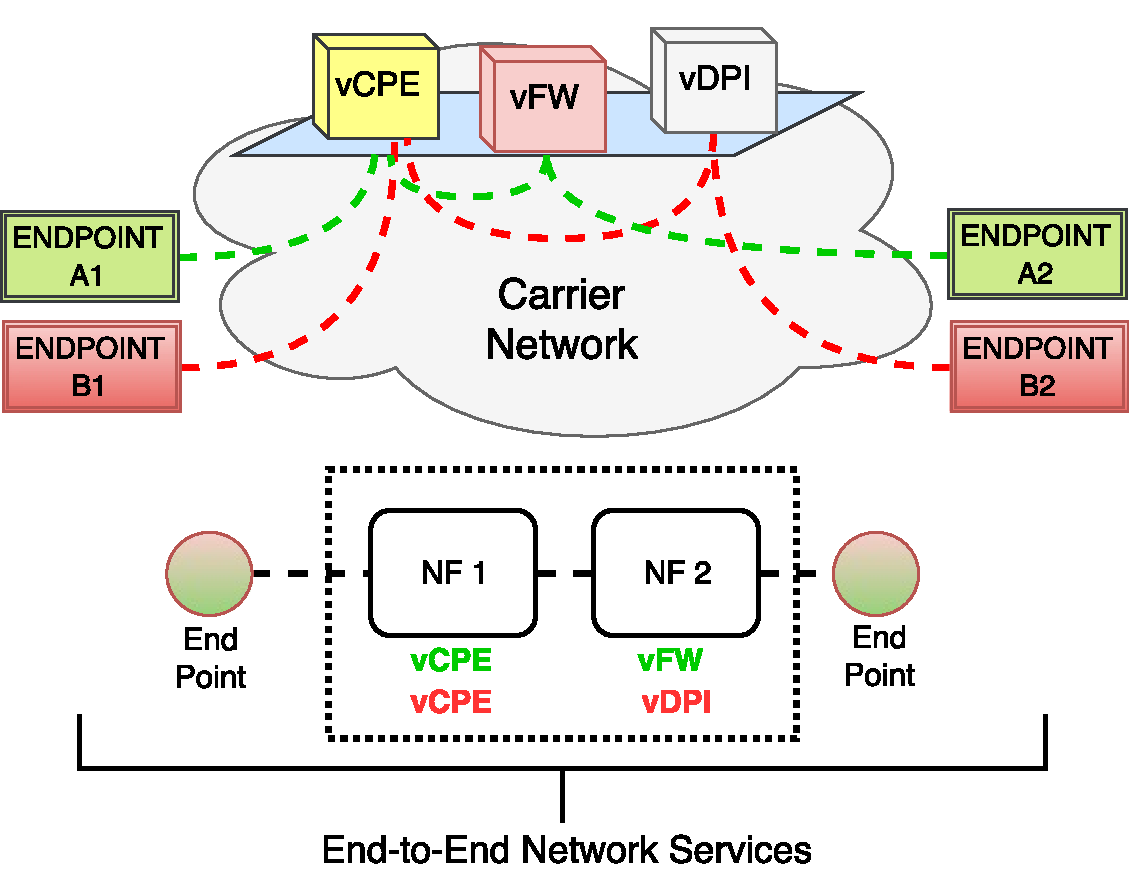
\includegraphics[scale=.45]{Figures/02_Background/ns}
    \caption{Example of two end-to-end network services composed of two \glspl{nf} each. NFV enables the reuse of \glspl{vnf}, e.g., \gls{vcpe}.}
    \label{nffg}
\end{figure}

\begin{figure}[t]
  \centering
  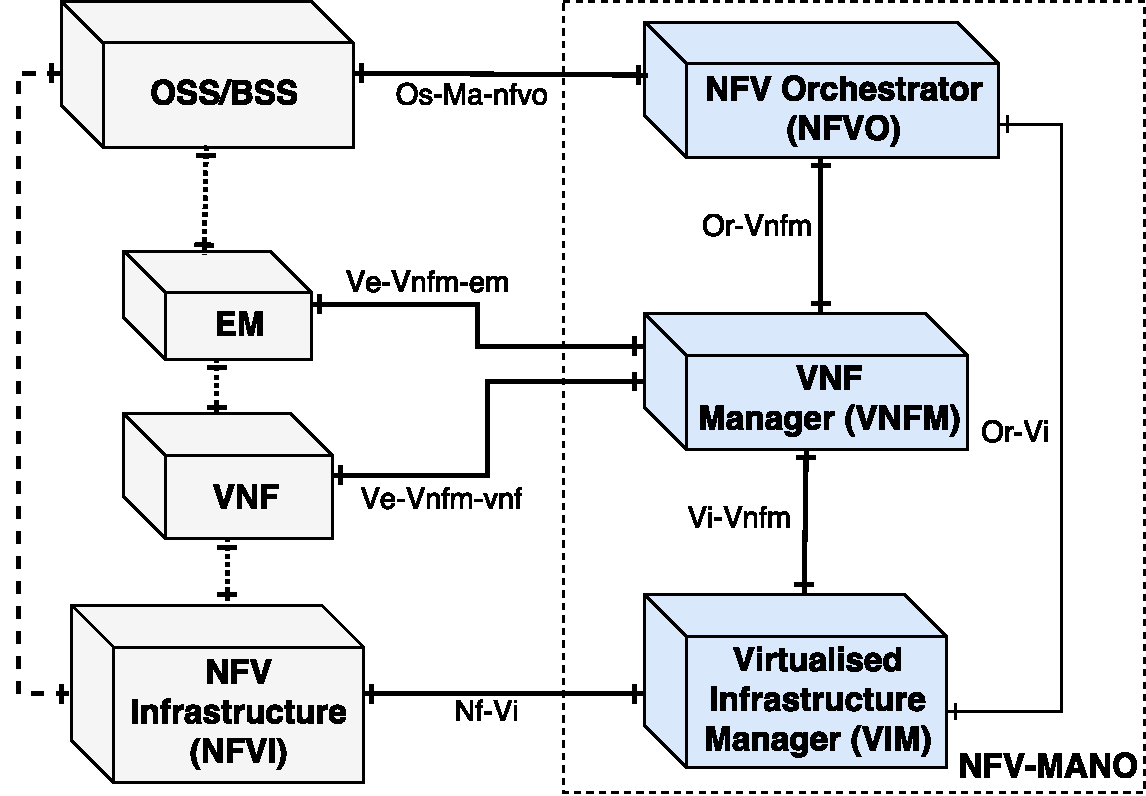
\includegraphics[scale=.4]{Figures/02_Background/MANO}
    \caption{The \gls{nfvmano} architectural framework. Adapted from \cite{ETSIIndustrySpecificationGroupISGNFV2014NetworkOptions}}
    \label{mano}
\end{figure}

The \gls{nfvmano} functional block performs all the virtualization-specific management, coordination, and automation tasks in the \gls{nfv} architecture including the components \gls{nfvo}, \gls{vnfm}, \gls{vim}, \gls{nfv} Service, \gls{vnf} Catalogue, NFV Instance, and \gls{nfvi} Resource. 

In the \gls{nfv} context, \gls{etsi} \gls{nfvmano} defines the orchestrator with two main functions including \textit{resources orchestration across multiple \glspl{vim}} and \textit{network service orchestration}~\cite{GSNFV-MAN001:2014}. Network service orchestration functions provided by the \gls{nfvo} are listed below:
\begin{itemize}
\item Management of Network Services templates and \gls{vnf} Packages. This includes validation of templates and packages with the objective of verifying the artifacts' authenticity and integrity. Besides, the software images are cataloged in involved \glspl{pop} using the support of \gls{vim}.
\item Network Service instantiation and management;
\item Management of the instantiation of \glspl{vnfm} and \glspl{vnf} (with support of \glspl{vnfm});
\item Validation and authorization of \gls{nfvi} resource requests from \gls{vnf} managers;
\item Management of network service instances topology;
\item Policy management related to affinity, scaling (auto or manual), fault tolerance, performance, and topology.
\end{itemize}

\gls{etsi} \gls{nfvo} functions regarding Resource Orchestration include: (\textit{i})  Orchestration of NFVI resources across multiple \glspl{vim}, (\textit{ii})  \gls{nfvi} resource management including compute, storage and network, and (\textit{iii}), collect usage information of \gls{nfvi} resources.
%\end{itemize}

The \gls{nfvmano} reference architecture is not  specific about \gls{sdn} in its architecture but  assumes that necessary transport infrastructure is already established and ready to be used. However, work at \gls{etsi} identifies use cases and the most common options for using SDN in an NFV architectural framework~\cite{ETSINetworkFramework}. The document also points to  proof of concepts and recommendations towards such integration work.
\cite{nfv-survey18} provides a recent in-depth survey on NFV state of affairs. 

%, from standardization to research. 
%Note that the \gls{etsi} only describes the functionalities of \gls{nfvmano} architecture and no defines regarding the technical details mainly to end-to-end network services. Moreover, there is no specification for the case where involves multiple networks with different technologies \cite{Katsalis2016Multi-DomainDirections}.

%Mateus: Does this subsection fit to background? 
%%%%%%%: Christian's Suggestion 
\subsection{Orchestration: Historical Overview}



%generic definition
The academic community and industry generally require some time to define the real meaning, reach and context of the concepts related to new technology trends as is the case with the term \textit{Orchestration}. 
The term orchestration is used in many different areas, such as multimedia, music, \gls{soa}, business processes, Cloud, \gls{sdn}, and, more recently, in \gls{nfv}.

%Maybe add about business process

From an end-user perspective, orchestration reminds a symphony orchestra where a set of instruments play together according to an arrangement. The music is arranged and split into small parts, after assigns to different musical instruments. When, who, and what will be played, as well as the conducting are essential parts towards achieving the desired effect. In next paragraphs, we identified the first works that use the orchestration in other areas. 

One of the first works in the \gls{ict} area that cites the term orchestration is \cite{Anderson1983} in 1983. It discusses that an autonomous system will require orchestration of the behavior of the entire system in order to obtain autonomy, interdependence and artificial intelligence. The authors in~\cite{Campbell1992} relate orchestration with the coordination and control of multiple media traffics. It distinguishes the orchestration from synchronization and defines an architecture where the orchestration acts in different layers. In the same scope, \cite{Robbins1997ImplementationArchitecture} relates the term to multimedia data, where orchestration is associated with multimedia presentation lifecycle management involving the coordination of stages that constitute all orchestration processes. 

The use of orchestration is also widely discussed in the scope of web services. In this context, orchestration and automation are considered separate processes. The work in~\cite{Peltz2003WebChoreography} defines orchestration like an executable process that can interact both internal and external services and must be dynamic, flexible, and adaptable to changes. It emphasizes that orchestration describe how web services can act with each other at the message level, including the business logic and execution order of the activities. 

The authors in~\cite{Grit2006} present the term orchestration in the context of virtual resource management. They define the orchestration as a process that involves all the necessary steps to map the application (running on a virtual machine) onto shared underlying infrastructure. 

%More recently in 2009, \cite{Galis2009ManagementInternet} provides an overview of 
Orchestration in the cloud environment is well-known and refers to locating, coordinating and selecting resources, including compute, storage and virtual networks to fulfill the desired requirements. The authors in \cite{Galis2009ManagementInternet} provide an overview of networking architecture definition for the \gls{fi} based on the concepts of cloud computing. One of the pillars for the \gls{fi} pointed out by the article is Orchestration. In the envisioned architecture, the orchestration function is to coordinate the integrated behavior and operations to dynamically adapt and optimize resources in response to changing context following business objectives and policies.

In the \gls{sdn} landscape, orchestration refers to an overarching function to manage and automate the network behavior~\cite{5984813}. %This means to govern all processes involved in the forwarding of network traffic. 
 More recently in 2012~\cite{ETSI2012NetworkAction}, orchestration has been generally related to \gls{nfv} environments mainly through its reference architecture and its \gls{nfv} Orchestrator component (more details in Subsection~\ref{subsec:nfv}).  

Currently, the scope of the orchestration has become broader and encompasses automation of the end-to-end network service lifecycle. According to \cite{MEF:Third:2015}, service orchestration refers to the programmatic control of underlying infrastructure including existing networks and enabling technologies, such as SDN and NFV.

%Orchestration in the cloud environment is well-known and refers to the locating, coordinating and selecting of resources, including compute, storage and virtual network, to fulfill the desired requirements \cite{Abosi2011}.   
%In short, the generalized orchestration means the capability to arrange, coordinate and manage systems, services, and resources in order to achieve an optimal outcome.

%%Orchestration is generally related to service automation in cloud~\cite{Abosi2011} and \gls{nfv} environments. In spite of that, its concepts are not clearly defined in the scope of \gls{nfv} yet \cite{Kuklinski2016DesignOrchestrators},~\cite{Alvizu2016AdvanceEra}. %Currently, this term is applied in network services deployment of telecommunication operators and service providers. 

From the existing and evolving definitions around orchestration presented, we can derive certain relationships between orchestration, automation, and management. Although the three terms are often lumped together, it is necessary an understanding of the differences between them as they are not the same thing. Automation describes a simple and technical task without the human intervention, for example, launching a web server, stopping a server. Management is responsible for maintaining and healthiness of infrastructure. Its role consists of activities such as alarms for event detection, monitoring, backups of critical systems, upgrades, and license management. Orchestration, in turn, is concerned with the execution of a workflow (processes) in the correct order. It controls the overall workflow process from starting the service until it ends with the objective to optimize and automate the network service deployment. 

Figure~\ref{diff} illustrates the relationship among orchestration, management, and automation. There is a certain hierarchic between them. The orchestration is a high-level plane, below the management, and in the bottom the automation. In our vision, the orchestration depends on tasks performed by management. Both management and orchestration are based on the use of automation in the execution of their tasks. Nevertheless, several activities are only performed by a certain function: optimization, for instance, cannot be achieved through simple automation. There is a difference between them, but, if they work together in the execution of processes, the services deployments will succeed with further accuracy.

\begin{figure}[t]
    \centering
    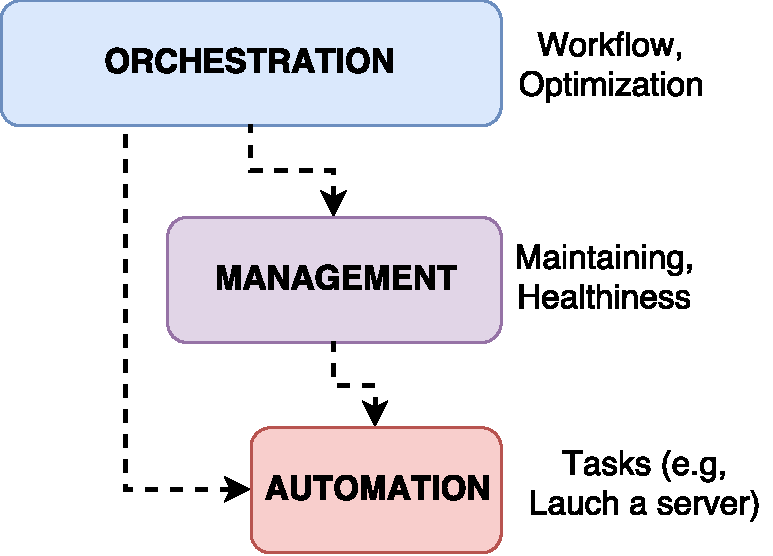
\includegraphics[scale=.45]{Figures/02_Background/OrchManaAut}
      \caption{Relationship among orchestration, management, and automation. Both orchestration and management use automation in their processes.}
      \label{diff}
\end{figure}

Based on all the above-mentioned background, in short, \gls{nso} is in charge of the full network service lifecycle to deliver end-to-end connectivity along additional services. To this end, orchestration is supported by advances in cloud computing, and technologies such as \gls{sdn} and \gls{nfv}, which offer the ability to reconfigure the network quickly as well as programming the forwarding and processing of the traffic. Figure~\ref{nso_rel} shows how \gls{nso}, \gls{nfv}, \gls{sdn}, and Cloud Computing work together. %Figure~\ref{nso_rel} aims at illustrating the relationships between \gls{nso}, \gls{nfv}, \gls{sdn}, and Cloud Computing.

Each one of these paradigms/technologies has different functions: high level orchestration for \gls{nso}, function programming for \gls{nfv}, networking programming for \gls{sdn},  and resource virtualization for cloud computing. Note that such technologies are complementary in order to provide complete management of the network services lifecycle. Although they have different functions, they share a common feature: \textit{orchestration}. They can work in an integrated pattern to offer advantages such as agility, cost reduction, automation, softwarization, and end-to-end connectivity, to enable novel services and applications such as 5G networks.

\begin{figure}[t]
  \centering
  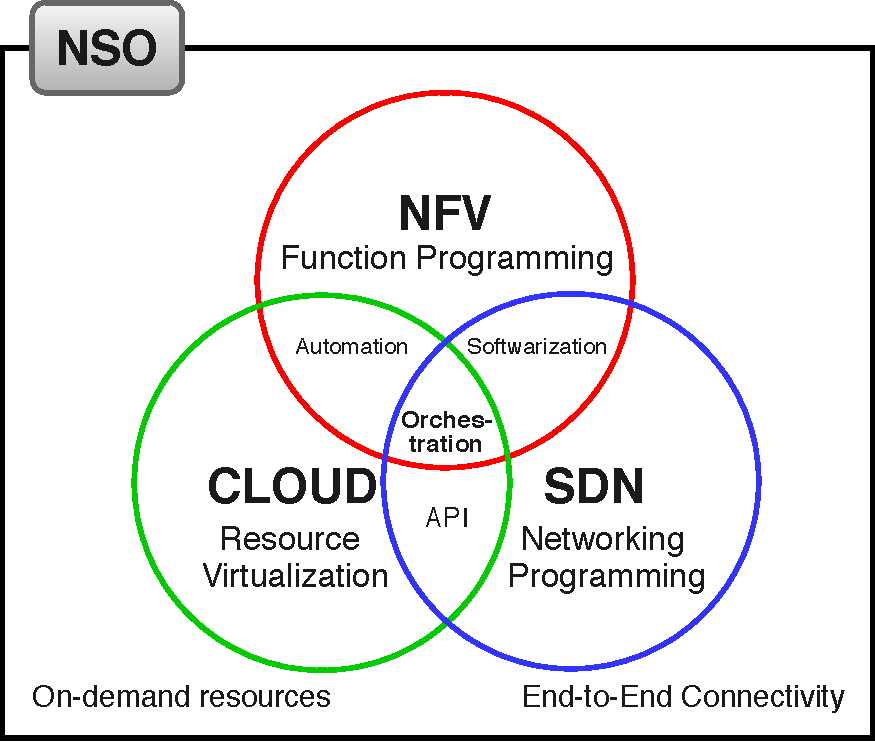
\includegraphics[scale=.45]{Figures/02_Background/nso_rel.pdf}
    \caption{Illustration of relationships among \gls{nso}, \gls{nfv}, \gls{sdn}, and Cloud.}
    \label{nso_rel}
\end{figure}

Our goal in this subsection was to set the ground and identify the main areas in which the term orchestration is inserted and how it is approached at a high level. An overview of the term usage is illustrated in the timeline of Table~\ref{timeline}. The focus of this survey is to detail the orchestration in the context of the implementation and operation of network services by operators and service providers.

\begin{table}[!]
\small
\caption{Historical timeline of term orchestration }\vskip -1ex
\label{timeline}
\begin{tabular}{@{\,}r <{\hskip 2pt} !{\foo} >{\raggedright\arraybackslash}p{5cm}}
\addlinespace[3ex]
\toprule
1983 & Autonomous system~\cite{Anderson1983}\\[13.5pt]
1992 & Media Traffic~\cite{Campbell1992}\\[7.5pt]
1997 & Multimedia presentation lifecycle management~\cite{Robbins1997ImplementationArchitecture}\\[1pt]
2003 & Web Service~\cite{Peltz2003WebChoreography}\\[4.5pt]
2006 & Virtual resource management~\cite{Grit2006}\\[4.5pt]
2009 & Cloud computing~\cite{Galis2009ManagementInternet}\\[3pt]
2011 & Software Defining Network~\cite{5984813}\\[1.5pt]
2012 & Network Function Virtualization~\cite{ETSI2012NetworkAction}\\[2pt]
2015 & Lifecycle Service Orchestration~\cite{MEF:Third:2015}\\
\end{tabular}
\end{table}


%\subsection{Relationship of Cloud, SDN, NFV, and NSO}

%%%%%% Improve the text about relevance of NSO %%%%%%% DONE




% \begin{figure}[t]
%     \centering
%     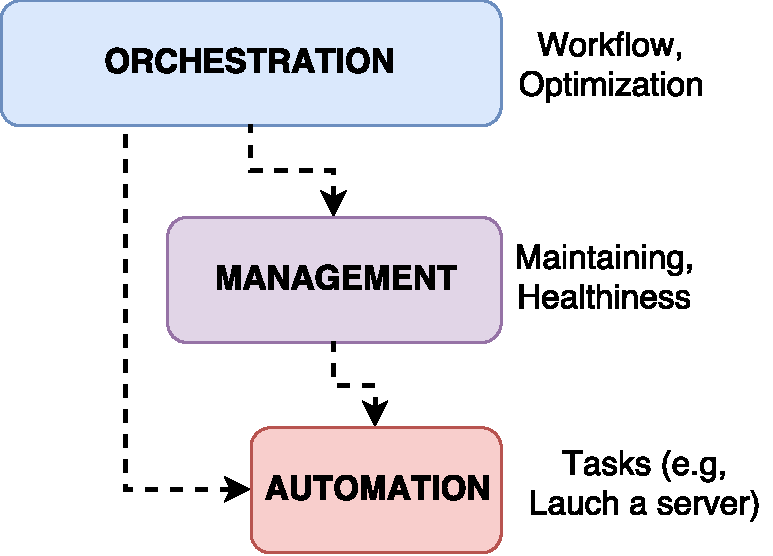
\includegraphics[scale=.4]{Figures/02_Background/OrchManaAut}
%       \caption{Relationship among orchestration, management, and automation. Both orchestration and management use automation in their processes.}
%       \label{diff}
% \end{figure}

%There is a difference between them but if they work together in the execution of processes, the services deployments will be successful and with further accuracy.


%%%%
%In short, the generalized orchestration means the capability to arrange, coordinate and manage systems, services, and resources in order to achieve an optimal outcome.

%Difference between orchestration and automation and management.
%ITU-T Y.3111
